\chapter{Implementation in the beamforming algorithm}
\label{chap:implementation}
\setheader{Implementation}

In this chapter the function which bridges between the experimental outcome and the beamforming algorithm will be described shortly.
At first the choice of returning impulse responses with a length of 1800 datapoints is discussed, where after the determination of the angles $\theta$ and $\phi$ between two places in space is explained.
With this functionality experiments have been conducted \cite{BAP:ErikNiels}, which results will be addressed shortly in the conclusion (Chapter \ref{chap:conclusion}).

\section{Functionality}
For the implementation of the directivity in the beamformer algorithm, the algorithm will call a function \texttt{directivity}, which will give an impulse response as result for given spacial locations.
This function is written in \matlab, to easily implement it in the beamforming algorithm, also written in {\matlab} \cite{BAP:ErikNiels}.
This impulse response will be transformed to the frequency domain by the algorithm, from which it will receive a gain for different frequencies.
This makes it easier for the algorithm to zero-pad or cut-off and so find the complex gains for the right frequencies.

The conducted measurements resulted in an impulse response vector with a length of approximately 32000 datapoints.
For the function to be quick, it needs as little memory communication as possible, next to that, the beamforming algorithm uses much less different frequency points  than the 16000 which can be computed with the result (about 2000 \cite{BAP:ErikNiels}).
Next to that, it is easy for the algorithm to use more different frequencies using zero-padding.

The powerspectrum of impulse responses for two different directions is given in Figure \ref{fig:impulse_length}. 
This impulse response is normalized to the maximum absolute value of the largest peak in all impulse responses for all directions for the {\nexus} labelled with number 6.
For the impulse response is a signal on which a convolution is performed, it can be read as all different Delta-peaks: they compute a delay and an attenuation of the original signal.

Very small Delta-peaks do not contribute to the impulse response, they are considered as noise: an attenuation of approximately -60 dB is inaudible by the human ear, when a normal sound level of a conversation of 60 dB is assumed \cite{hospital}, therefore all peaks smaller than -60 dB can be ignored.
In the figure can be seen that after approximately 1500 datapoints (or 0.03 seconds) both signals are below the -60 dB line, datapoint from this point are insignificant. 
For some certainty 1800 datapoints are outputted to the beamforming system.

\section{Determining angles}
To meet the requirements given in Appendix \ref{app:requirements}, the function should give an impulse response for a given $\theta$ and $\phi$.
For convenience and to avoid mistakes in different spherical coordinate-systems, another function is written, which has as input two places in space (the place of the smartphone $(\mathbf{p}_p)$ and the place of the source $(\mathbf{p}_s)$) and which solves the problem of determining $\theta$ and $\phi$.

Using the inner product \cite[p.~21]{book:poole} \eqref{eq:innerproduct}, the angle between two vectors can be determined.
Taking the phone as the origin of the Cartesian coordinate system, the angle between the $x$-axis and the $(x,y)-$vector pointing from the phone towards the source results in $\theta$ \eqref{eq:theta}.
And in the same way, the angle between the $z$-axis and the $(x,z)$-vector pointing from the phone towards the source results in $\phi$ \eqref{eq:phi}.

After the determination of the angles, making use of the \texttt{load}-function in in {\matlab} to only read one vector in the memory, the impulse response for the given places in space is returned.

\begin{eqnarray}
\label{eq:innerproduct}
\langle\mathbf{a},\mathbf{b}\rangle&=&\|\mathbf{a}\|\|\mathbf{b}\|\cos\theta\qquad\text{with }\theta\text{ the angle between }\mathbf{a}\text{ and }\mathbf{b}\\
\mathbf{p}&=&\left[\begin{array}{c}
p^x\\
p^y\\
p^z
\end{array}\right]=\mathbf{p}_s-\mathbf{p}_p\\
\label{eq:theta}
\theta&=&\arccos\left(
\dfrac{\left\langle\left[\begin{array}{c}
p^x\\
p^y
\end{array}\right],\left[\begin{array}{c}
1\\
0
\end{array}\right]\right\rangle}
{\left\|\left[\begin{array}{c}
p^x\\
p^y
\end{array}
\right]\right\|}
\right)\\
\label{eq:phi}
\phi&=&\arccos\left(
\dfrac{\left\langle\left[\begin{array}{c}
p^x\\
p^z
\end{array}\right],\left[\begin{array}{c}
0\\
1
\end{array}\right]\right\rangle}
{\left\|\left[\begin{array}{c}
p^x\\
p^z
\end{array}
\right]\right\|}
\right)
\end{eqnarray}

\vspace{1in}

\begin{figure}[h!]
	\centering
	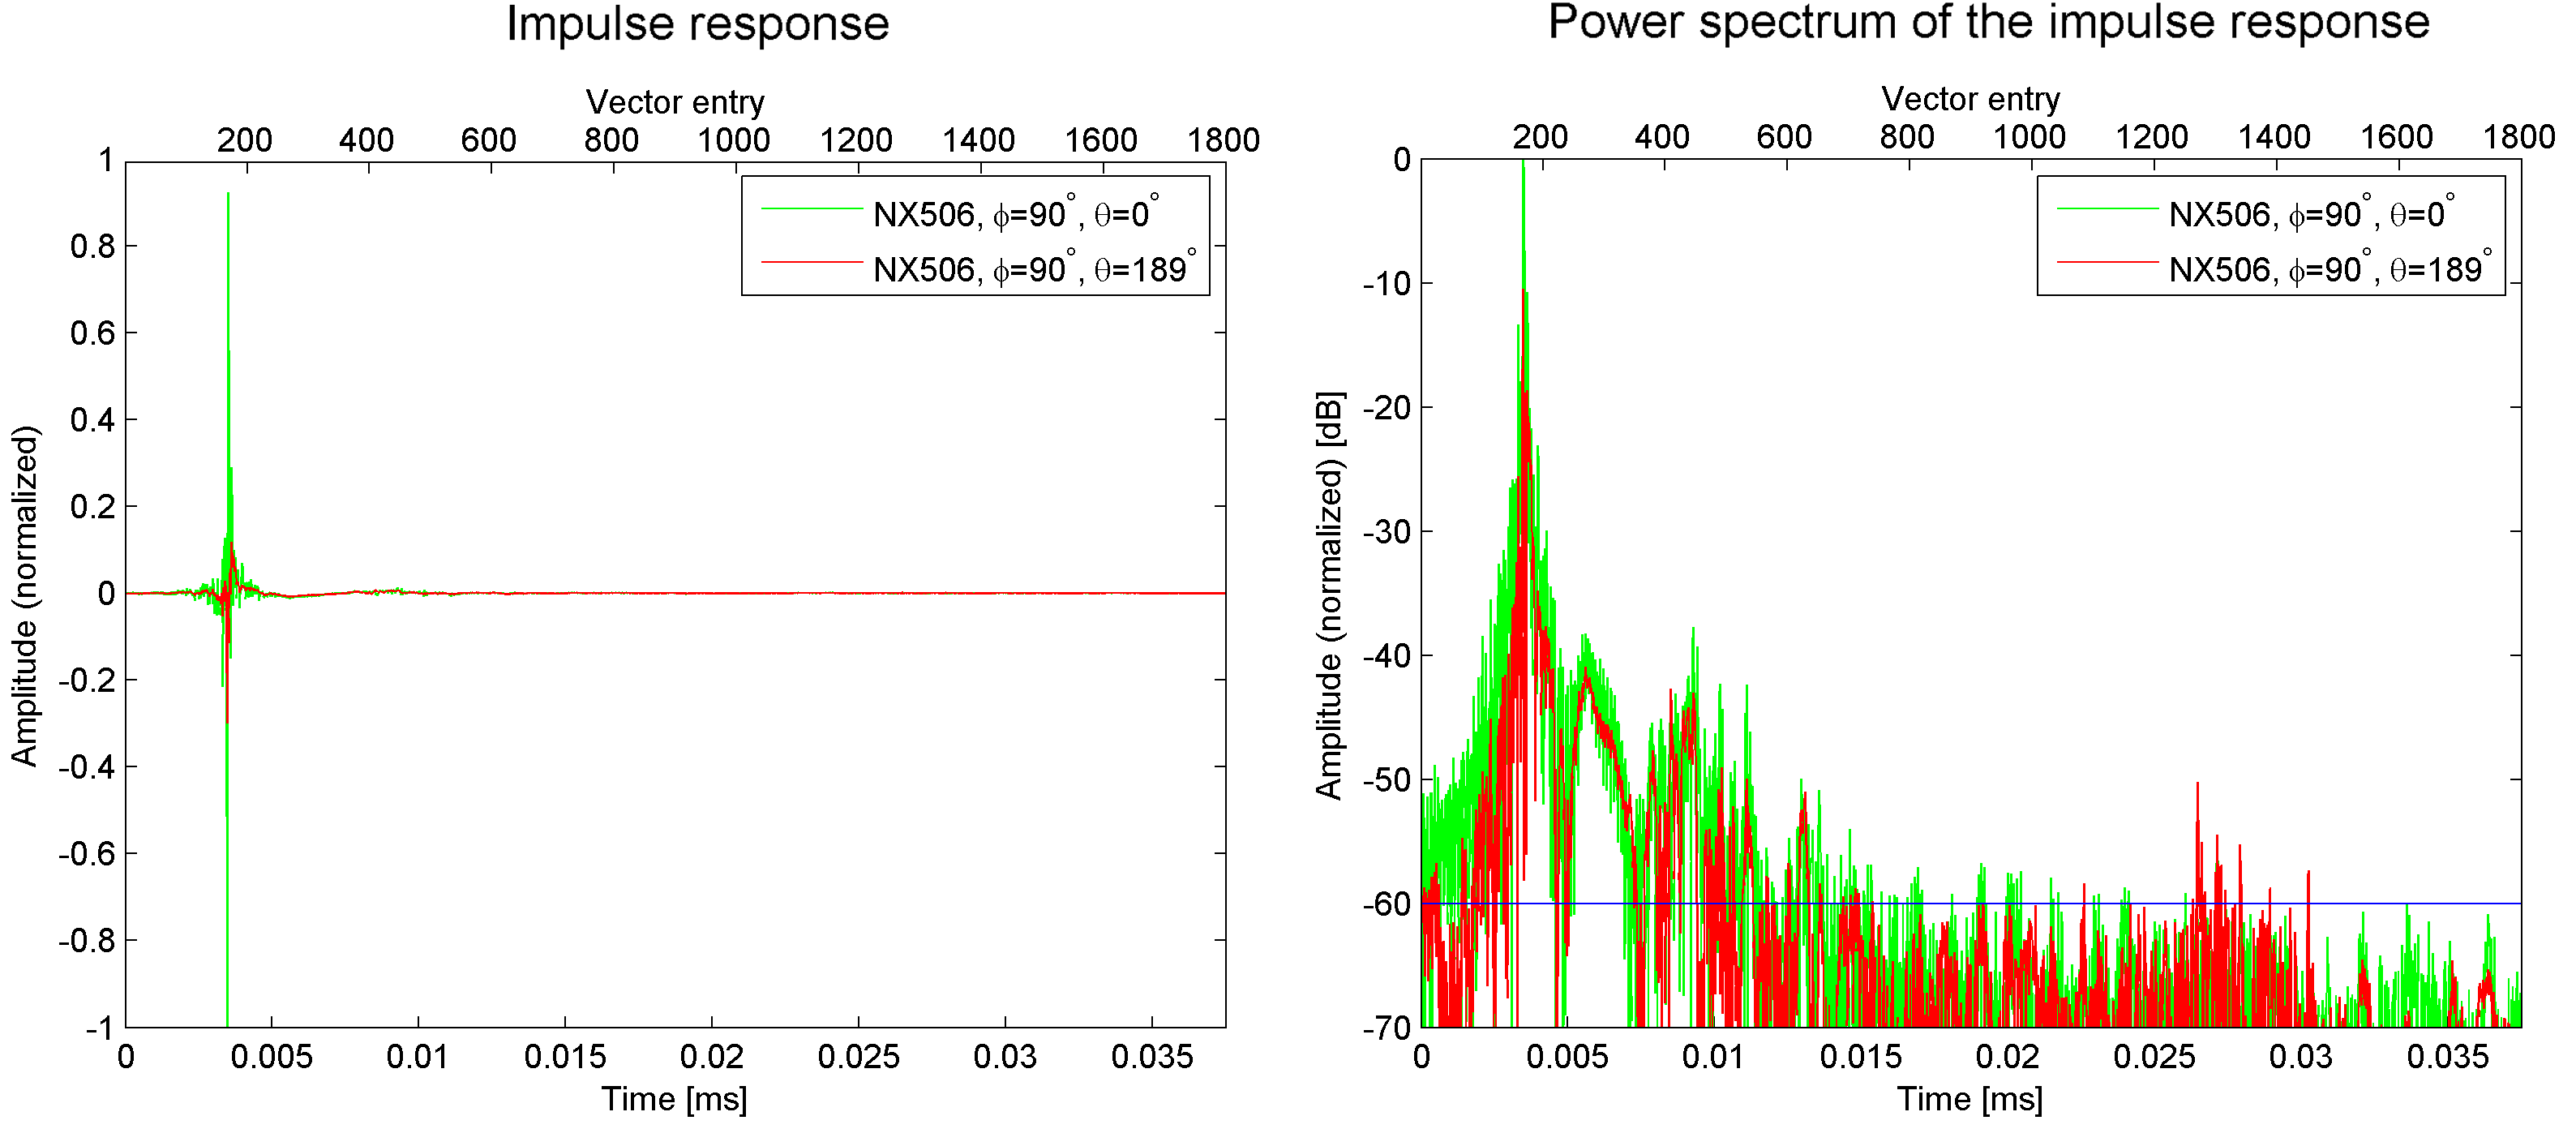
\includegraphics[width=\textwidth]{afbeeldingen/plots/impulse_response_length.png}
	\caption[Impulse response in decibel-domain]{The impulse response of two different measurements in the dB-domain. The blue line denotes the -60 dB line from the highest point.}
	\label{fig:impulse_length}
\end{figure}